\documentclass[11pt, oneside]{article}
\usepackage{geometry}
\geometry{letterpaper}
\usepackage{graphicx}
\usepackage{amssymb}
\usepackage{amsmath}
\usepackage{tikz}
\usepackage{tikz-qtree}
\usepackage{url}
\usepackage[T1]{fontenc}

\title{SICP Exercise 3.36}
\author{Yuchong Pan}

\begin{document}
\maketitle

The environment in which \textbf{(for-each-except setter inform-about-value constraints)} is evaluated is given as follows.

\begin{figure}[h!]
    \centering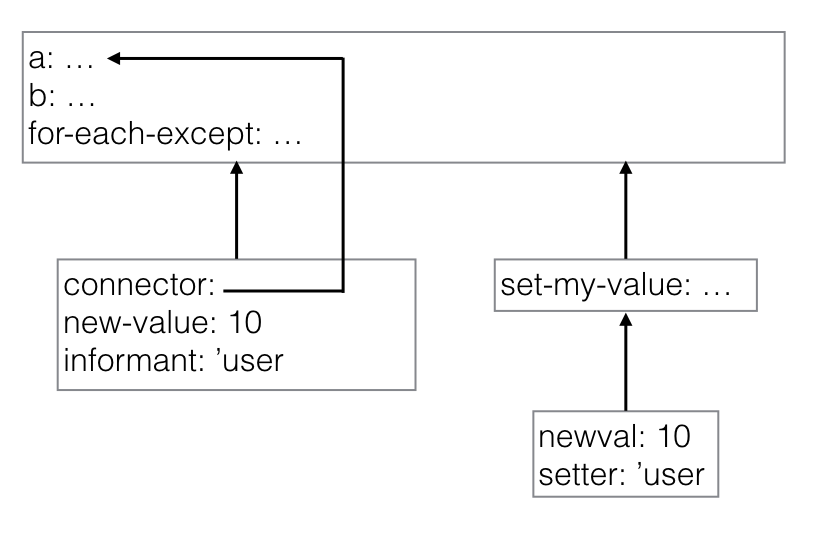
\includegraphics[width=15cm]{ex-3.36.png}
    \caption{The environment in which the expression is evaluated.}
\end{figure}

\end{document}
